\documentclass[11pt,usenames,dvipsnames]{beamer}

\usepackage{tikz}
\usepackage{graphicx}
\usepackage{natbib}
\usepackage{bibentry}
%\usepackage{ctable,tabularx,array}
\usepackage{subfig}
\usepackage{grffile}
\usepackage{amssymb,amsmath}
\usepackage[english]{babel}
\usepackage[latin1]{inputenc}
%\usepackage[orientation=landscape,size=a0,scale=1.25,debug]{beamerposter}
\usepackage[orientation=portrait,size=a0,scale=1.1,debug]{beamerposter}
\usepackage{caption}
%\usepackage{caption}

%\usepackage[parfill]{parskip}    % Activate to begin paragraphs with an empty line rather than an 
\setlength{\parskip}{10pt}
\usepackage{cinzel}
\usepackage{heuristica}
\usepackage[default,regular,black]{sourcesanspro}
\usepackage[default,regular,black]{sourcecodepro}

\usepackage[T1]{fontenc}


%\usefonttheme{professionalfonts} % using non standard fonts for beamer
%\usefonttheme[onlymath]{serif} % default family is serif

\usetheme{Sam}

\def\wordcol#1{%\left\{%
\tabcolsep=0pt%
\mbox{%
%\renewcommand{\baselinestretch}{2}
\def\arraystretch{1}%
\small %\sl%
\begin{tabular}{c}%
%\textnormal{#1}%
#1
\end{tabular}%
}%end mbox
%\right\} 
}%end wordcol

\renewcommand{\thefootnote}{}
\def\newblock{\hskip .11em plus .33em minus .07em}
\renewcommand{\vec}[1]{\mbox{\boldmath{$#1$}}}
\newcommand{\mat}[1]{\mathrm{#1}}


\title[]{Visualisation of random effects\\[12pt] in Bayesian hierarchical models}
\author{Sam Clifford \and You, the Reader}
\institute{Science and Engineering Faculty, Queensland University of Technology, Brisbane, Australia}
\date{}

\begin{document}

%\input{columns.tex}
\frame{
\begin{columns}
 \begin{column}[t]{0.45\linewidth}
%  \begin{block}{Abstract}
  \begin{block}{Introduction}
\setlength{\parskip}{15pt}

Communication of parameter values and predictions is an important part of presenting the results of statistical modelling, whether via graphical means or numerical summaries. With the popularity of Bayesian modelling software such as WinBUGS \citep{WinBUGS2000}, JAGS \citep{jags03, jags} and STAN \citep{STAN2017}, it has become common to show trace plots and density plots when presenting analysis as these are the default visualisations shown by the coda package in R \citep{CODA}. Those writing their own samplers, whether in R, MATLAB, C++ or some other language must also make choices about how to present their results and are no doubt influenced by common approaches from other software. The more complex the model, the more complex the visualisation task, particularly when considering hierarchical models with mixed effects across multiple levels.

\end{block}

\begin{block}{An anthology}
\setlength{\parskip}{15pt}

The WinBUGS software is many practitioners' first exposure to Bayesian modelling. Its use of density and trace plots as the basis for visually considering parameter samples results in the, perhaps undeserved, passing on of these visualisation techniques as the standard technique. As models grow both in the number of observations and the complexity of the parameter hierarchy, there is a need to do better in communicating the credible intervals of parameters and the values these parameters take within a level of the hierarchy.


The coda functionality from S+ was ported to be an R package in 1999, providing a way to interact with MCMC samples in R. While very useful in terms of being able to assess the convergence of the Markov chains in the model, the plot methods which provide trace and density plots for the samples do poorly in terms of presenting meaningful information.

Due to the long history of these code bases, the difficulty of changing the direction of well-established software and the fact that no one seems to beating down the doors of the WinBUGS/OpenBUGS developers to force them to focus on visualisation, little has been done to modify the visual tools available to BUGS users in R with the exception of making use of trellis graphics.

The STAN software, and its R interface, go some way to reducing the amount of space dedicated to trace plots and density plots by summarising parameter estimates with credible intervals with levels 0.8 and 0.95 and showing posterior medians. This provides for visualiation which is closer to Tufte's idea of maximising the data:ink ratio but can often lead to excess whitespace when parameter values are on different scales \citep{tufte1983visual}.

The rise of the tidyverse package family \citep{tidyverse} has resulted in the ggmcmc package \citep{ggmcmc}, an implementation of coda style visual summaries in the ggplot2 grammar of graphics framework \citep{ggplot2}. While this results in a more elegant framework for visualisation, such a framework does not guarantee easily interpretable presentation of complex information, nor does it guarantee that the visualisation engages the reader. Using ggplot2 to reproduce coda graphics is like 3D printing lipstick directly on to the proverbial pig.

\end{block}

\begin{block}{Tables}
\setlength{\parskip}{15pt}
	
Looking back even further, an alternative to providing graphical summaries of parameter estimates is to provide a table of means, medians and other summary statistics in a table. This quickly becomes unwieldy for large sets of parameters, and making comparisons becomes nearly impossible as the number of numbers on the page grows.
	
\end{block}

 \begin{block}{Model and data}
	\setlength{\parskip}{15pt}
	
	The data are the rats data set, commonly used as a WinBUGS demonstration, giving the weight of 30 rats at 5 evenly spaced times after birth \citep{Gelfand1990}.
	
	The model is a linear model with random effects for the slope and intercept for each rat's growth trajectory,
	
	\begin{minipage}{0.45\linewidth}
		
		\begin{align*}
		y_{ij} \sim & \, N \left( \mu_{ij}, \tau \right) \\
		\mu_{ij} = & \, \beta_{0i} + \beta_{1j} \, x_{ij} \\
		\beta_{0j} \sim & \, N \left( \beta_{00}, \tau_0 \right) \\
		\beta_{1j} \sim & \, N \left( \beta_{10}, \tau_1 \right) \\
		\beta_{00}, \beta_{10}  \sim & \, N \left( 0, 10^{-6} \right) \\
		\tau , \tau_0, \tau_1 \sim & \, \Gamma\left( 0.001, 0.001 \right)
		\end{align*}
		
	\end{minipage}\quad
	\begin{minipage}{0.45\linewidth}
		
		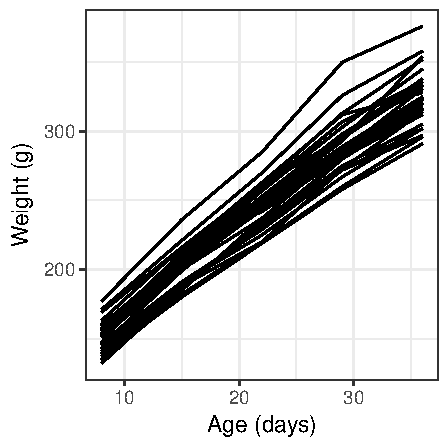
\includegraphics[width=\linewidth]{data.pdf}
		
	\end{minipage}
	
\end{block}



\begin{block}{Methodology}
	
	\setlength{\parskip}{15pt}
	
	You are invited to provide feedback on the following graphs by placing a coloured sticker on or near each of them, corresponding with your opinion. \textcolor{ForestGreen}{\bfseries Green} -- I like this plot.  \textcolor{Goldenrod}{\bfseries Yellow} -- I am ambivalent or indifferent about this plot.  \textcolor{Red}{\bfseries Red} -- I dislike this plot. Paper is provided in order for you to provide your own idea for visualisation after discussing what you like or dislike about each approach.
	
\end{block}

\end{column}

 \begin{column}[t]{0.45\linewidth}
 


\begin{block}{Visualisations}
	\setlength{\parskip}{15pt}

%\begin{figure}
%\includegraphics[width=0.8\linewidth]{trad}
%\caption{Posterior medians and 95\% credible intervals}
%\end{figure}

\begin{figure}
	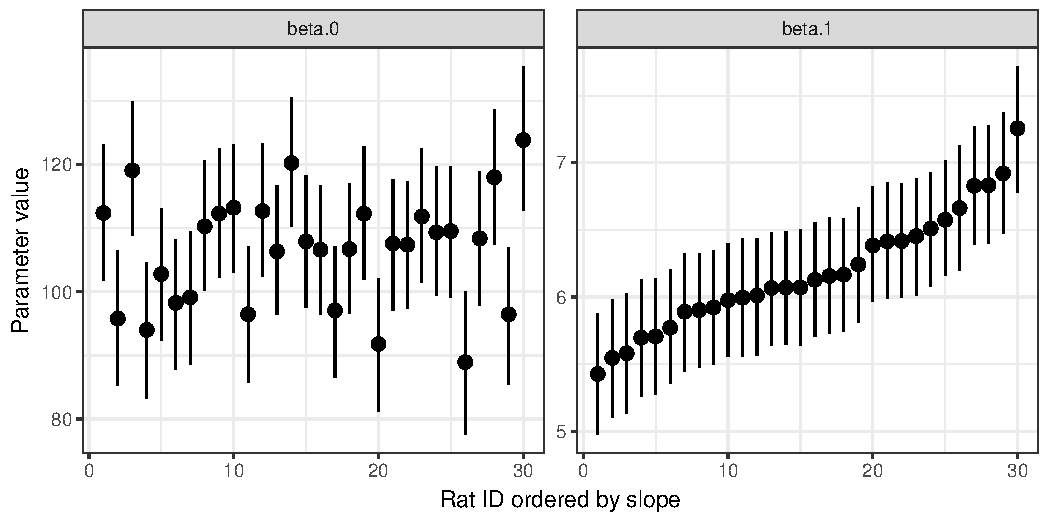
\includegraphics[width=0.8\linewidth]{raterpillar}
	\caption{Caterpillar plot of medians and 95\% credible intervals}
\end{figure}

\begin{figure}
	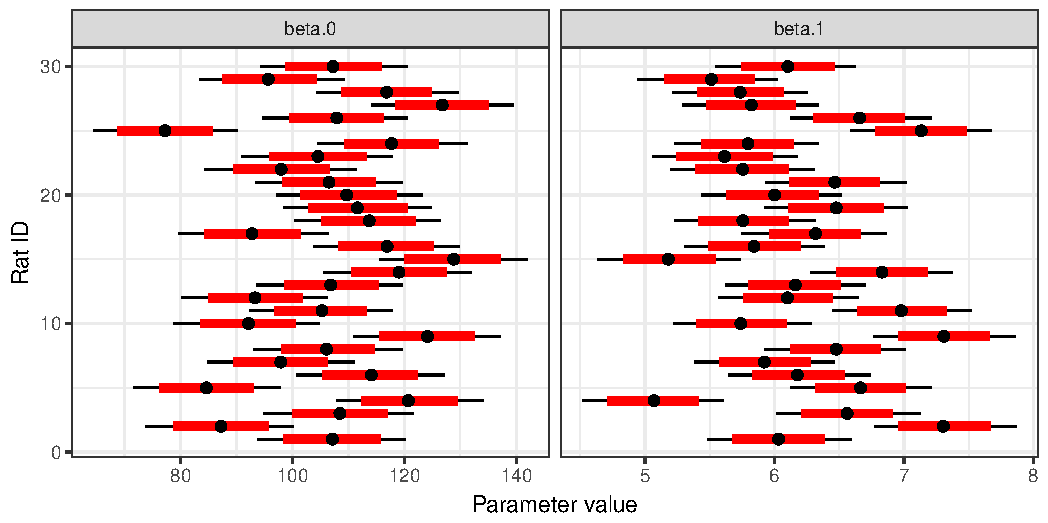
\includegraphics[width=0.8\linewidth]{stan}
	\caption{Medians, 80\% and 95\% credible intervals (a la STAN)}
\end{figure}

\begin{figure}
	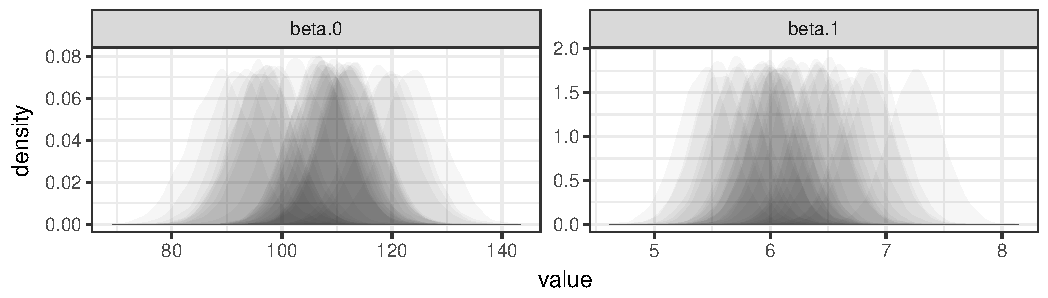
\includegraphics[width=0.8\linewidth]{ghost}
	\caption{Density plots of random effects (filled) and distribution of means (outline)}
\end{figure}

\begin{figure}
	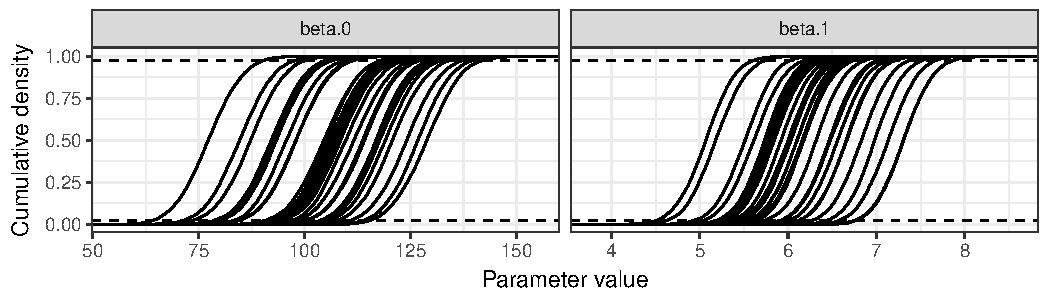
\includegraphics[width=0.8\linewidth]{aitkin}
	\caption{Cumulative density plots}
\end{figure}


\begin{figure}
	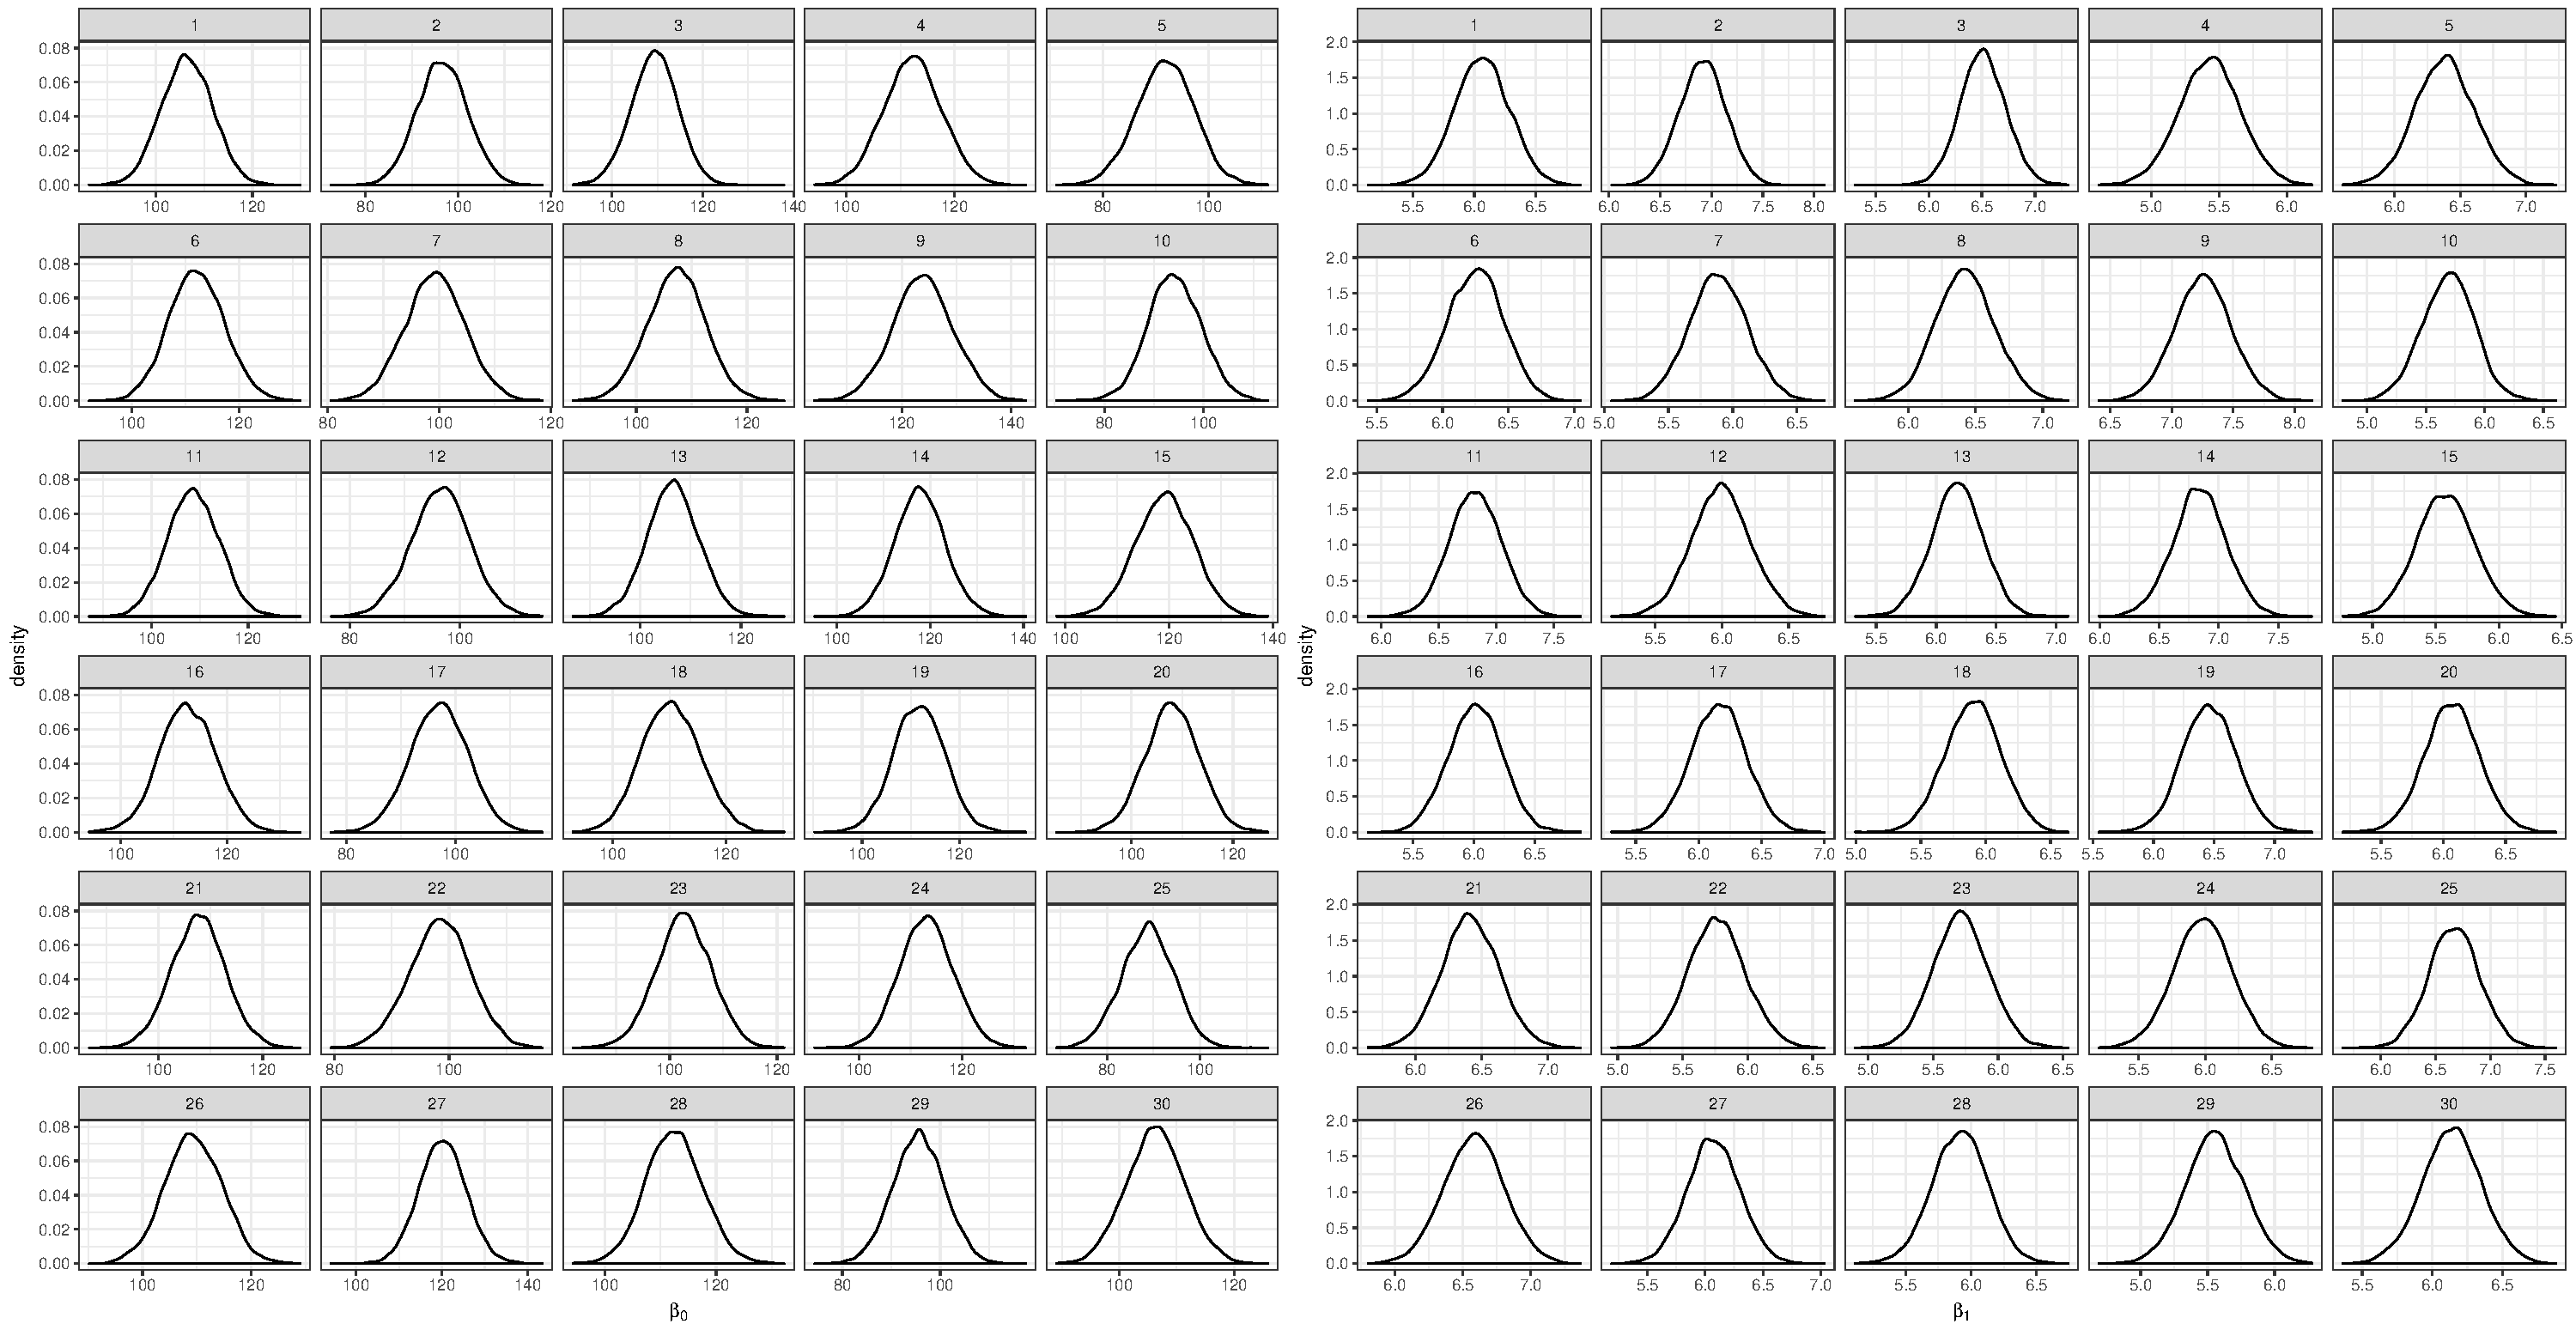
\includegraphics[width=0.8\linewidth]{winbugs}
	\caption{Small multiples of density plots}
\end{figure}


\end{block}

\begin{block}{References}
\setlength{\parskip}{15pt}

\footnotesize

\bibliographystyle{chicago}
\bibliography{botb}

\end{block}
 \end{column}
\end{columns}

}



\end{document}
